%filename: troubleshooting.tex
\section{故障排查}

\begin{frame}{故障排查}

目标
\begin{itemize}
\item 研制一套故障排查策略
\item 修复Linux不同领域故障
\item 启动系统到不同runlevel
\item 使用救援(Resuce)环境
\end{itemize}
\end{frame} 

\subsection{故障分析}



\begin{frame}{故障分析方法}
\begin{itemize}
\item 问题特征化
\item 重现问题
\item 挖掘更多信息
\item 排除可能原因
\item 首先尝试容易的事情
\item 改变前备份配置文件
\end{itemize}

\end{frame} 
\begin{frame}{故障分析:收集信息}
\begin{itemize}
\item 有用的命令

\begin{itemize}
\item history 
\item grep
\item diff
\item find \emph{/dir} -cmin -60
\item strace \emph{command }
\item tail -f \emph{logfile}
\end{itemize}
\item 产生额外的信息

\begin{itemize}
\item syslog.conf里加入{*}.debug项
\item 应用程序尝试--debug 选项
\end{itemize}
\end{itemize}
\end{frame} 

%\subsection{X 检查}
%
%\begin{frame}{X 检查事项}
%\begin{itemize}
%\item 不在runlevel 5模式下调试X
%\item 如果硬件改变,首先尝试system-config-display
%\item X
%\item /home 或 /tmp 空间满了?或者是达到磁盘配额上限?或者是/tmp权限问题?
%\item xfs在运行吗?
%\end{itemize}
%\end{frame} 


\subsection{网络检查}

\begin{frame}{网络检查事项}
\begin{itemize}
\item 主机名解析
	\begin{itemize}
	\item dig www.redflag-linux.com
	\end{itemize}
\item IP 配置
	\begin{itemize}
	\item ifconfig
	\item ip
	\end{itemize}
\item 缺省网关
	\begin{itemize}
	\item route -n
	\item ip route show
	\end{itemize}
\item 特定内核模块
\item 设备激活
\end{itemize}
\end{frame} 


\begin{frame}{系统启动顺序}
\center
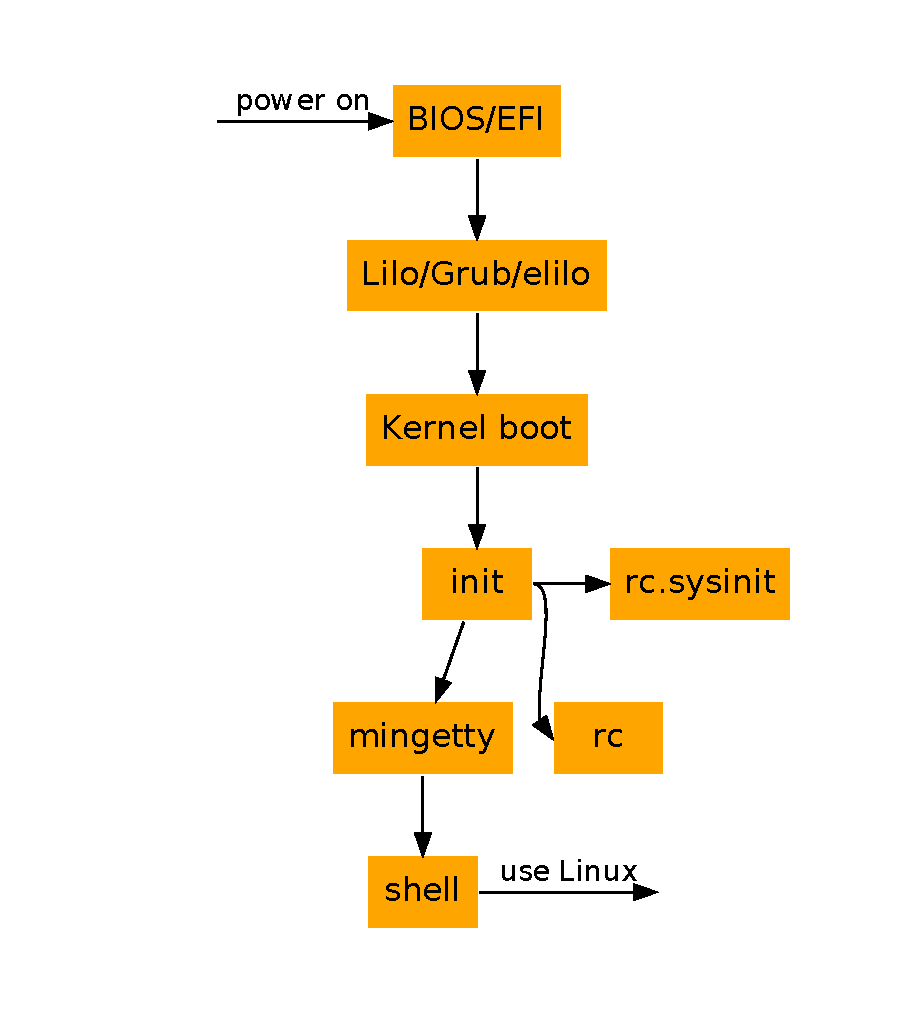
\includegraphics[height=.8\textheight]{images/boot.pdf}

%\begin{itemize}
%\item 加载器配置文件(/boot/grub/grub.conf)
%\item Kernel
%\item /sbin/init
%\item /etc/rc.d/rc.sysinit
%\item etc/rc.d/rc,/etc/rc.d/rc?.d/
%\item /etc/rc.d/rc.local
%\item X
%\end{itemize}
\end{frame}


\subsection{文件系统故障}



\begin{frame}{启动时的文件系统问题}
\begin{itemize}
\item rc.sysinit 尝试挂载本地文件系统
\item 如果失败,引导至root shell环境(需要输入密码)

\begin{itemize}
\item fsck 可以用来修复损坏的文件系统
\item 运行fsck之前

\begin{itemize}
\item 检查/etc/fstab是否有错误
\item 手工测试挂载文件系统
\end{itemize}
\end{itemize}
\end{itemize}

\end{frame} 
\begin{frame}{文件系统损坏}
\begin{itemize}
\item 一般系统崩溃或者非正常关机会导致文件系统损坏
\item 标记为`dirty'的ext2文件系统挂载时:

\begin{itemize}
\item 如果没有挂载或者只读挂载,标记为`clean'
\item 如果没有挂载且标记为`dirty',可能会报文件系统损坏
\item 需要彻底检查文件系统来进行修复
\end{itemize}
\item ext3通常标记为`clean'

\begin{itemize}
\item 如果需要恢复,日志(journal)会指出这点
\item 需要检查记录在日志里的文件
\end{itemize}
\end{itemize}

\end{frame} 
\begin{frame}{文件系统恢复}
\begin{itemize}
\item 如果 / 是日志文件系统,系统启动时检查它
\item /etc/rc.d/rc.sysinit 对/etc/fstab标记需要检查的文件系统做检查
\item fsck是其他文件系统检查工具的前端程序
\item fsck检查失效,则必须手工干预和执行
\end{itemize}

\end{frame} 
\begin{frame}{恢复运行级别}
\begin{itemize}
\item 传递运行级别(run-level)给init

\begin{itemize}
\item 在grub引导时传递参数
\item 在命令行下,使用init/telinit来改变
\end{itemize}
\item Runlevel 1

\begin{itemize}
\item 处理 rc.sysinit和rc1.d/目录下的脚本
\end{itemize}
\item Runlevel s/S/single

\begin{itemize}
\item 仅处理 rc.sysinit
\end{itemize}
\item emergency

\begin{itemize}
\item 仅处理sulogin
\end{itemize}
\end{itemize}
\end{frame} 

\subsection{救援环境}

\begin{frame}{救援环境}
\begin{itemize}
\item 当根文件系统失效时可以用到它
\item 非系统特性
\item 从第一张系统安装光盘启动,或者boot.iso
\item 如果是U盘,从diskboot.img启动
\item 引导后出现boot: 的地方,输入\alert{linux rescue}
\end{itemize}

\end{frame} 
\begin{frame}{工具}


\begin{itemize}
\item 磁盘维护工具
\item 网络工具
\item 其他一些工具
\item 记录日志: /tmp/syslog 或 /tmp/anaconda.log
\end{itemize}

\end{frame} 
\begin{frame}{细节}
\begin{itemize}
\item 文件系统重新组织

\begin{itemize}
\item anaconda 将会询问你是否需要挂载
\item /mnt/sysimage/{*}
\item /mnt/source
\item \$PATH 包括了磁盘的目录
\end{itemize}
\item 文件系统设备

\begin{itemize}
\item 提供特定文件系统设备
\item mknod可以创建已知主设备号和次设备号的设备
\end{itemize}
\end{itemize}
\end{frame} 


%\subsection{系统救援和故障排查实验}
%
%\begin{frame}{实验I:救援模式下修复GRUB}
%
%
%\begin{description}
%\item [{场景:}] 救援环境提供了修复机器不能启动的最后手段,即便引导器或者根文件系统损坏或者配置错误都可以修复。现在,有一台服务器在引导时,仅出现GR提示符,无法引导系统。请修复它。
%\end{description}
%提示
%\begin{itemize}
%\item 模拟MBR错误
%\item 第一张光盘引导,输入linux rescue
%\item 使用grub-install 指令
%\end{itemize}
%
%\end{frame} 
%
%\begin{frame}{实验II:救援模式下安装软件}
%
%
%\begin{description}
%\item [{场景:}] 因为文件系统的损坏,导致/bin/下的关键可执行程序损坏,包括/bin/mount,/bin/bash等。导致系统无法启动,请你修复该系统。
%\item [{要求:}] 修复损坏的RPM包
%\end{description}
%提示
%\begin{enumerate}
%\item 了解损坏的文件属于哪个RPM包
%\item 进入救援模式
%\item chroot环境
%\item 重新安装包
%\end{enumerate}
%\end{frame}
